\documentclass{beamer}

\usepackage{graphicx}

\title{Learning to Classify Useful Reviews}
\author{Ertan Dogrultan \and Cesar Romero \and Paul Wais\\
% Computer Science Department \\
% University of California, Los Angeles\\
% Los Angeles, California 90095\\
\texttt{\{ertan,romero,pwais\}@cs.ucla.edu}}
\date{November 29, 2010}
\begin{document}
\maketitle{}

\begin{frame}{User Votes Inform Review Sorting and Search}
\begin{figure}[h]
  \centering
  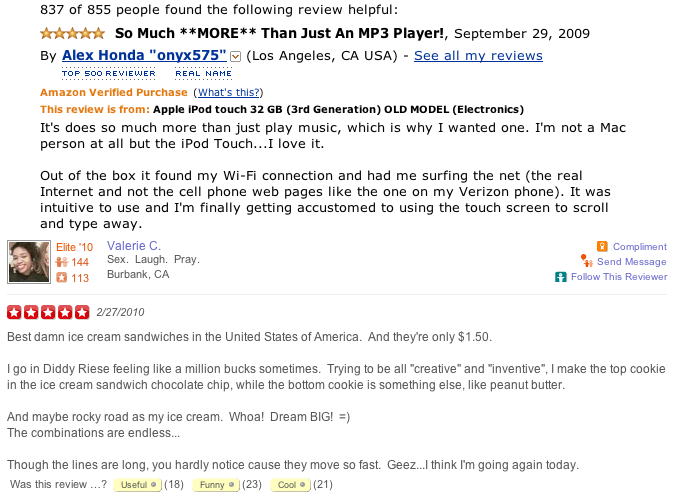
\includegraphics[scale=.4]{review_ex_1}
\end{figure}
\end{frame}

\begin{frame}{Unfortunately, votes are sparse ...}
\begin{figure}[h]
  \centering
  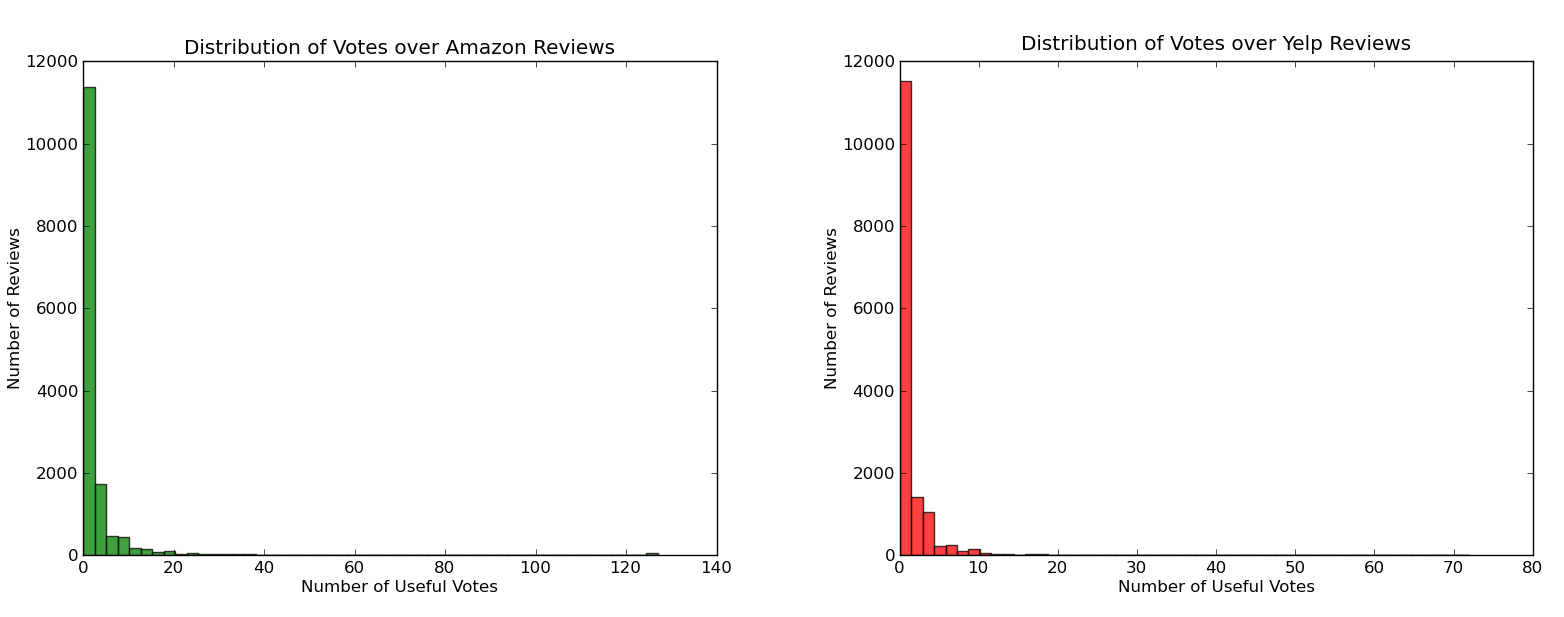
\includegraphics[width=\linewidth]{histos}
  \label{fig:histos}
\end{figure}
\end{frame}

\begin{frame}{... and there are many useful (and not so useful) reviews without votes}
\begin{figure}[h]
  \centering
  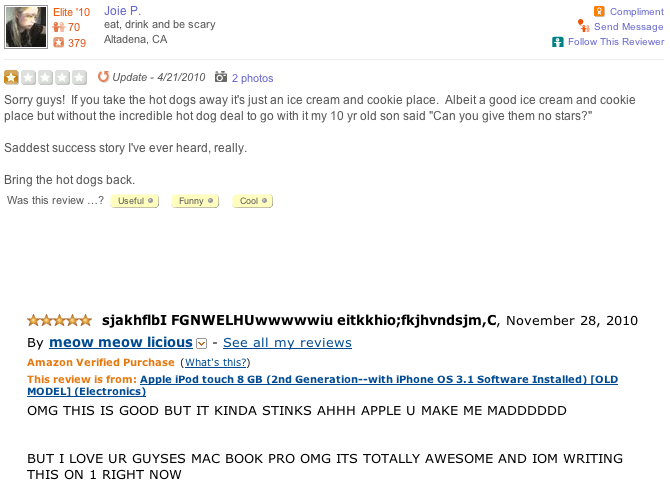
\includegraphics[scale=.4]{review_unvoted}
  \label{fig:unvoted}
\end{figure}
\end{frame}

\begin{frame}{Goal: Learn to Classify Reviews as Useful (or Not)}
\begin{figure}[h]
  \centering
  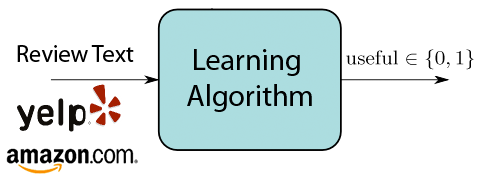
\includegraphics[scale=.4]{learning_summary}
  \label{fig:summary}
\end{figure}
\begin{itemize}
\item Corpus: 15,000 Yelp and Amazon reviews annotated with ``useful'' vote counts. \footnote{{\tiny We thank Yelp, Inc., and Aditya Mukherji (CMU '11) for help in obtaining data for this project.}\\}
\item Test a variety of algorithms: SVM, Naive Bayes, AdaBoost, Winnow.  Why does one algorithm outperform others?
\item Also investigate domain adaptation: e.g. apply Yelp-trained model to Amazon reviews.
\end{itemize}
\end{frame}

\begin{frame}{Note: Usefulness is Independent of Sentiment}
\begin{figure}[h]
  \centering
  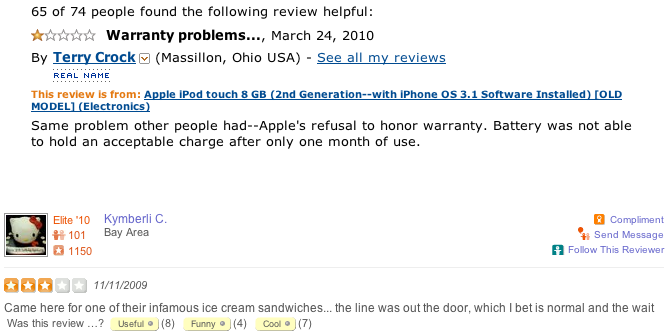
\includegraphics[scale=.4]{review_ex_2}
\end{figure}
\begin{itemize}
\item Pang et al. \footnote{{\tiny Pang, Bo and Lillian Lee and Shivakumar Vaithyanathan.  "Thumbs
up?  Sentiment Classification using Machine Learning Techniques."
Proceedings of the 2002 Conference on Empirical Methods in Natural
Language Processing (EMNLP). 2002}} test Maximum Entropy, Naive Bayes, and SVM models for classifying sentiment and achieve about 80\% accuracy.\\
\end{itemize}
\end{frame}


\begin{frame}{Features for Classifying Usefulness}
\begin{itemize}
\item Frequencies of ANEW\footnote{{\tiny Sheridan Dodds, Peter and Christopher M. Danforth. "Measuring the Happiness of Large-Scale Written Expression: Songs, Blogs, and Presidents."  Journal of Happiness Studies, Volume 11, Number 4, 441-456, DOI: 10.1007/s10902-009-9150-9. }} words, GRE/SAT words, logical signposting phrases, $\ldots$ 
\begin{itemize}
\item For example: ``love'' has valence 8.72; ``rude'' has valence of 2.5
\end{itemize}
\item Frequencies of grammatical errors, typpppos, capitalization IrReGuLARIties, $\ldots$
\item URLs, IDF Scores of n-grams, product or business price, $\ldots$
\end{itemize}
\end{frame}

\begin{frame}{Feature Distributions}
\begin{figure}[h]
  \centering
  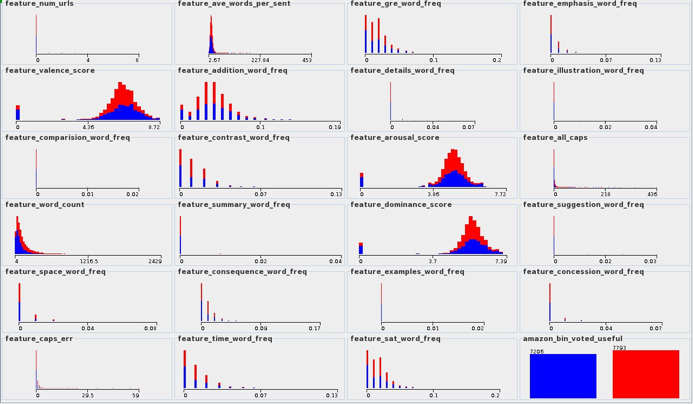
\includegraphics[scale=.4]{features_distributions}
  \caption{The distributions of the features}
  \label{fig:dist}
\end{figure}
\end{frame}

\begin{frame}{Cross-validation accuracy of the algorithms}
\begin{table}[ht]
  \centering
  \begin{tabular}{c | c}
    Algorithm    & Accuracy \\
    \hline
    SVM (RBF)    & 70.13\%  \\
    SVM (Linear) & 75\%     \\
    Adaboost     & 80\%     \\
    Naive Bayes  & 68.5\%   \\
    Winnow       & 56\%     \\
  \end{tabular}
  \caption{The 10 fold cross-validation accuracy of the algorithms}
  \label{tab:performance}
\end{table}
\end{frame}

\begin{frame}{Complications}
Why do different algorithms perform differently on this task?
\begin{itemize}
\item SVM
\item Adaboost
\item Naive Bayes 
\end{itemize}
\end{frame}

\begin{frame}{Future Work}
\begin{itemize}
\item Domain adaptation experiments
\begin{figure}[ht]
\centering
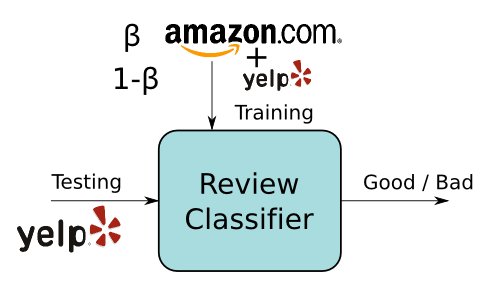
\includegraphics[scale=.3]{adaptation}
\label{fig:adaptation}
\end{figure}
\item Connections with the theoretical bounds
\end{itemize}

\end{frame}
\end{document}
